%% 
%% Copyright 2007, 2008, 2009 Elsevier Ltd
%% 
%% This file is part of the 'Elsarticle Bundle'.
%% ---------------------------------------------
%% 
%% It may be distributed under the conditions of the LaTeX Project Public
%% License, either version 1.2 of this license or (at your option) any
%% later version.  The latest version of this license is in
%%    http://www.latex-project.org/lppl.txt
%% and version 1.2 or later is part of all distributions of LaTeX
%% version 1999/12/01 or later.
%% 
%% The list of all files belonging to the 'Elsarticle Bundle' is
%% given in the file `manifest.txt'.
%% 

%% Template article for Elsevier's document class `elsarticle'
%% with numbered style bibliographic references
%% SP 2008/03/01

%\documentclass[preprint,12pt]{elsarticle}

%% Use the option review to obtain double line spacing
%% \documentclass[authoryear,preprint,review,12pt]{elsarticle}
%%  \documentclass[2014,preprint,review,12pt]{elsarticle}

%% Use the options 1p,twocolumn; 3p; 3p,twocolumn; 5p; or 5p,twocolumn
%% for a journal layout:
% \documentclass[final,1p,times]{elsarticle}
%% \documentclass[final,1p,times,twocolumn]{elsarticle}
%% \documentclass[final,3p,times]{elsarticle}
%% \documentclass[final,3p,times,twocolumn]{elsarticle}

%% \documentclass[final,5p,times,twocolumn]{elsarticle}

%% For including figures, graphicx.sty has been loaded in
%% elsarticle.cls. If you prefer to use the old commands
%% please give \usepackage{epsfig}

%% The amssymb package provides various useful mathematical symbols

%% The amsthm package provides extended theorem environments
%% \usepackage{amsthm}

%% The lineno packages adds line numbers. Start line numbering with
%% \begin{linenumbers}, end it with \end{linenumbers}. Or switch it on
%% for the whole article with \linenumbers.
%% \usepackage{lineno}

%% Title, authors and addresses

%% use the tnoteref command within \title for footnotes;
%% use the tnotetext command for theassociated footnote;
%% use the fnref command within \author or \address for footnotes;
%% use the fntext command for theassociated footnote;
%% use the corref command within \author for corresponding author footnotes;
%% use the cortext command for theassociated footnote;
%% use the ead command for the email address,
%% and the form \ead[url] for the home page:
%% \title{Title\tnoteref{label1}}
%% \tnotetext[label1]{}
%% \author{Name\corref{cor1}\fnref{label2}}
%% \ead{email address}
%% \ead[url]{home page}
%% \fntext[label2]{}
%% \cortext[cor1]{}
%% \address{Address\fnref{label3}}
%% \fntext[label3]{}


%% use optional labels to link authors explicitly to addresses:
%% \author[label1,label2]{}
%% \address[label1]{}
%% \address[label2]{}

% % % % % % % % % % % % % % % % % % % % % % % % % % % % % % % % % % % % % % % % % % % % % % % % % %
% % % % Preamble
% % % % % % % % % % % % % % % % % % % % % % % % % % % % % % % % % % % % % % % % % % % % % % % % % %
\documentclass[final,5p,times]{elsarticle}
\usepackage{amssymb}
\usepackage{amsmath}
\usepackage{epsfig}
\usepackage{url}
\usepackage{float}
\journal{International Journal of Impact Engineering}
%\hyphenation{*LOAD\_-BLAST\_-ENHANCED}
\begin{document}
% % % % % % % % % % % % % % % % % % % % % % % % % % % % % % % % % % % % % % % % % % % % % % % % % %
% % % % Frontmatter (Authors/Abstract/Keywords)
% % % % % % % % % % % % % % % % % % % % % % % % % % % % % % % % % % % % % % % % % % % % % % % % % %
\begin{frontmatter}
%\title{Numerical modelling of the structural response of welded materials under complex loading configurations. %panels subjected to air blast.
%Part I: Numerical modelling}
\title{Finite element based modelling of the structural response of welded materials in complex loading configurations. %panels subjected to air blast.
Part I: Structural modelling considerations}
\author[1]{A.J. Awang Draup \corref{cor1}}
\ead{jefri.draup@postgrad.manchester.ac.uk}
\author[1]{J.D Robson}
\author[1]{P.B. Prangnell}
\author[1]{Q.M. Li}
\address[1]{The University of Manchester, Manchester, M13 9PL, UK}
\author[2]{M.J. Lunt}
\address[2]{DSTL, Porton, SP4 0JQ, UK}
\cortext[cor1]{Corresponding author. Tel: +44 (0)161 306 3578 Ext. 2261}

\begin{abstract}
This two-part article presents the results of numerical  prediction and experimental studies which aim to determine the structural response of friction stir welded aluminium 2139-T8 subjected to complex loading configurations, and in particular, air blast loading. The aim of this work is to develop a numerical modelling methodology to allow detailed prediction of the local strain evolution across the weld zone as this has significant influence in relation to structural response and failure. In particular, the method allows local material property gradients, which are due to variation in strengthening mechanism arising from microstructural damage caused by thermal loading during the welding process, to be incorporated into a macro scale structural model. Part I details the methodology used to implement local material property gradients together with experimental evidence to verify the predicted structural response in a range of loading configurations. Part II provides an insight into the assumptions made in Part I with respect to high strain rate materials modelling across the weld zone and the associated evidence for the variation in strengthening mechanisms in the alloy. The work presented highlights the importance of accurate description of the variation in local material properties, particularly the work hardening rate, in determining the response of structures under blast loading.
\end{abstract}

\begin{keyword}
%% keywords here, in the form: keyword \sep keyword
Blast loading\sep Digital image correlation \sep Materials modelling \sep Finite element simulation \sep Materials characterisation
%% PACS codes here, in the form: \PACS code \sep code
%% MSC codes here, in the form: \MSC code \sep code
%% or \MSC[2008] code \sep code (2000 is the default)
\end{keyword}

\end{frontmatter}

% % % % % % % % % % % % % % % % % % % % % % % % % % % % % % % % % % % % % % % % % % % % % % % % % %
% % % % Introduction
% % % % % % % % % % % % % % % % % % % % % % % % % % % % % % % % % % % % % % % % % % % % % % % % % %
\section{Introduction}
\label{Intro}
%
%Weld modelling of blast of interest.\\Particularly case of failure/performance. \\ Application is plastic collapse of buildings, failure in structures.\\Typical methods in litereature
%subject to assumptions which induce error, require careful calibration and interpretation.\\Particular important details are geometry, loading etc\\WRT mat props there is major simplification. typical approach\\implications in terms of range of model validity\\Propose a more detailed approach 
The structural performance of welded structures subjected to air blast loading is of key interest to engineers and scientists across a range of industries. For civilian applications, typically the risk of air blast is due to gas explosions and is an important design consideration in the construction of offshore oil platforms \cite{Langdon2005,Langdon2005a,Langdon2006}. %; 
%Other areas include the risk of gas ingress and explosion in domestic properties. 
%another consideration may be the risk of terrorist attack using explosives in public buildings. 
A key consideration here is not necessarily just the initial damage from the blast loading, but the risk of subsequent injury from collapse of the remaining structure. For steel framed buildings that are common in civil engineering, plastic deformation in the joints, which may be manufactured by welding, can be the limiting factor controlling structural integrity \cite{Ngo2007}. Detailed understanding of this localised damage is extremely important when considering the potential resistance of a building to blast and, therefore, any required mitigating engineering works to reinforce the structure; this may have an impact on the cost or design layout of a structure.
For military applications, the use of welded joints is common in personnel transport vehicles. With an increase in the threat from Improvised Explosive Devices (IEDs), the performance of welded structures has come under scrutiny \cite{Ramasamy2011}. There has been a global trend towards the use of vehicles, such as the Mastiff, which are designed to be mine resistant \cite{Morse2011}. In critical areas of a typical vehicle, such as the underbelly, the use of monolithic structures has become favourable as welds may lose integrity under blast loading. Local failure in the weld can lead to ingress of the explosive shock front into the vehicle, which can have catastrophic consequences on the occupants of the vehicle \cite{Ramasamy2011}. Indeed, it is unsurprising that one area of current research focus is on predictive techniques to aid the understanding of deformation and failure mechanisms in welded structures subjected to blast loading \cite{McWilliams2013,Grujicic2011a,Grujicic2012}.
Of course, in order to model the non-linear behaviour of a welded structure accurately, it is necessary to understand the interrelation between materials processing, material microstructure and the subsequent material and mechanical properties. Furthermore, the application of numerical modelling techniques, alongside the intrinsic errors arising due to the modelling assumptions made, need to be fully understood if a high fidelity model of weld behaviour is to be utilised and interpreted correctly.
%TODO Decide where this chunk of information should be put!
The scope of this paper limits discussion to structures manufactured via Friction Stir Welding (FSW), as described in \S\ref{IntroFSW}. Furthermore, discussion will be limited to heat treatable aluminium alloys, with particular reference to the alloy 2139-T8 as described in \S\ref{IntroAluminium2139t8}, though the general concepts are applicable across other alloys. Finally, consideration is only given to the Finite Element Method (FEM), as described in \S\ref{IntroWeldeModelling}, since it is widely used as a tool to study the response of structures under a wide range of loading conditions.

\subsection{Aluminium 2139-T8}
\label{IntroAluminium2139t8}
%A bit about the alloy
%particular strengthening mechanisms
%Gradual and distinct changes in the properties due to strengthening mechanisms
%Particular effects which impact definition of properties that are important to FE modelling
%In this work, we focus on the aluminium alloy 2139-T8. 
Originally developed for aerospace applications demanding high fracture toughness and fatigue life at elevated temperatures, the alloy demonstrates superior performance at elevated temperatures and strain rates in comparison to existing alloys \cite{Cho2006,Vural2009}. The alloy has also been found to demonstrate superior ballistic performance in comparison to existing armour alloys \cite{Vural2009,Grujicic2010a}. As a result, there is interest in using this alloy for military vehicle applications as an alternative armour alloy. 2139-T8 is an Al-Cu-Mg-Ag based alloy whose composition leads to the preferential formation of the stable $\Omega$ phase \cite{Bakavos2008,Lee2010,Elkhodary2011b}:
\begin{equation*}
\begin{split}
\text{SSSS} & \rightarrow  \text{GPZ} \rightarrow \theta''\rightarrow \theta' \\
& \rightarrow \Omega
\end{split}
\end{equation*}
The $\Omega$ phase forms as extremely fine, hexagonal plate-like precipitates oriented along the natural slip planes of the aluminium crystal structure, $\text{\{111\}}_\mathrm{\alpha}$; precipitate spacing in the T8 condition is of the order 10\textsuperscript{1} nm. Whilst this alloy does contain other secondary phases, such as manganese and zirconium containing particles, it is widely accepted that $\Omega$ is the dominant phase in the T8 condition and, therefore, precipitation hardening due to the $\Omega$ phase is the major strengthening mechanism to the alloy. Hence, the mechanical properties of 2139-T8 are sensitive to variation, in terms of size and distribution, of the $\Omega$ phase. In Part II, Transmission Electron Microscopy (TEM) is used to gain an understanding of the variation in strengthening mechanism in FSW 2139-T8 by observing the effects of FSW on the $\Omega$ phase and a more in depth discussion shall be given there. Briefly, the $\Omega$ phase responds to the local thermal cycle experienced during FSW. Heat input during processing may cause the $\Omega$ phase to overage and coarsen; if temperatures are high enough the $\Omega$ phase may go into solution. Therefore, FSW may cause significant local changes to the strengthening mechanisms in 2139-T8. This process is relatively well understood and can be predicted using existing methods in the literature. 
\subsection{Friction Stir Welding}
\label{IntroFSW}
%What FSW is
%what are the typical impact on the material (weld zones)
%for aluminium 
First described in 1991 by TWI, FSW is a solid state joining process which enables the manufacture of high quality joints in materials that are difficult to manufacture via traditional fusion based techniques, such as 2xxx and 7xxx aluminium alloys \cite{Karlsson2000,Peel2003}.  FSW has the advantage of reducing both the thermal degradation to the parent material microstructure and the residual stress generated during manufacture in comparison to fusion based joining methods \cite{Mishra2005}. These advantages make the technology suitable for the manufacture of welded structures from alloys such as 2139-T8. 
In FSW, the tool, which is comprised of a rotating pin and shoulder, is used to generate frictional heat in the work-piece. This source of heat softens the material locally around the tool which can then be mechanically mixed about the tool as it rotates and traverses the joint line of the workpiece. Since the process induces a temperature rise that is below the melting temperature of the alloy, the welding occurs in the solid state. 
Whilst there is no physical state transformation, diffusional transformation processes can occur which significantly affect the properties across the weld zone. These processes are alloy specific but generally they induce certain meso-scale features in the weldzone. These features include the formation of a Heat Affected Zone (HAZ); a Thermo-Mechanically Affected Zone (TMAZ), and a central region known as the Nugget which is approximately enveloped by the dimensions of the tool itself \cite{Mishra2005}. Within each region there exists strong material property gradients; these gradients are linked to the induced changes in microstructure, which can locally alter the strengthening mechanisms from that which controls the parent material \cite{Su2003,Mahoney1998}. 
For heat treatable aluminium alloys, in addition to the intrinsic strength, mechanisms such as precipitation hardening from second phase particles, solute hardening, grain size hardening, and work hardening all contribute to the overall strength of a material. In the HAZ, softening is due to thermal loading arising during the welding process alone; softening processes include coarsening and dissolution of strengthening precipitates. In the TMAZ, there are additional mechanisms which arise due to the interaction of mechanical processes. For example, large deformation may be induced in the alloy which may affect the contribution from grain size. In the nugget region, the large amount of heat and plastic strain is enough to induce dynamic recrystallisation in the alloy. In this region, grain size and distribution are an important contributing factor to the properties of the material. Since the local material properties are controlled by these changes in strengthening mechanisms \cite{Karlsson2000}, it is necessary to develop an understanding of how they develop during welding in order for them to be incorporated into any structural model to study weld performance.

%In order to define the local material properties accurately, it is necessary to understand what the strengthening mechanisms are, and these tend to be alloy specific.
\subsection{Weld Modelling}
\label{IntroWeldeModelling}
The typical method to study structural response to loading is to use the FEM and there are many instances of its use to study the response of welded structures \cite{Grujicic2011,McWilliams2013,Reis2004,Zhao2001}. However, successful macro scale modelling of weld behaviour under general loading conditions is extremely challenging as there are many factors which contribute to the overall structural behaviour. In addition to the variation in strengthening mechanisms across the weld zone (\S\ref{IntroFSW}), phenomena such as geometry misalignment from the welding process, the formation of weld defects, and residual stresses are all complexities which contribute to structural performance \cite{Kim2010,Grujicic2011a}. For example, residual stresses are known to adversely affect the fatigue life of welded structures. Moreover, correct application of modelling technique, such as definition of loading and boundary conditions are pertinent to model quality.  Whilst there has been a lot of work to improve FE based modelling methods with respect to some of the afore mentioned phenomena, a systematic approach to implementing local material property variation which arise due to welding process, which provides close quantitative correlation between prediction, has not emerged in the public domain. 
%there can be influence from local geometry variations due to misalignment of the welded plates or weld flash alongside complex residual stress fields induced by the welding process. Moreover, physical processes which occur on a micro scale significantly influence the material properties local to the weld zone, thereby generating structural variation and complexity on a meso-scale. 
In FEM based modelling, meso-scale complexity is typically dealt with by partitioning the mesh into distinct regions, which are representative of the weld regions (i.e. Nugget, TMAZ, HAZ and parent material) \cite{McWilliams2013,Grujicic2011}. Elements are assigned to these partitions and are collectively assigned homogeneous isotropic properties; these are usually defined by a Johnson-Cook material model:
\begin{equation}
\label{eq1}
\sigma = \bigg( A + B\epsilon^n_{p} \bigg)\; \bigg(1 +C\,\text{ln}\bigg(\frac{\dot{\epsilon}_{p}}{\dot{\epsilon}_{p0}}\bigg)\bigg)\; \bigg(1-\bigg(\frac{T-T_0}{T_m-T_0}\bigg)^m\bigg)
\end{equation}
It is common to assume that all parameters in equation \ref{eq1} are the same as the parent material except for the A parameter; this is assumed to scale linearly with hardness. The geometry of each region, such as the HAZ, may be defined by examination of the hardness distribution in the cross section of an actual weld or by visual inspection of metallographic specimens. However, it is common practice to calibrate the geometry of the model to experimental data from a real weld loaded in uniaxial tension. Usually, the calibrated model is extended to more complex structures and loading configurations without any further modifications \cite{McWilliams2013,Grujicic2011a}. This approach will hereby be referred to as the "lumped-mass" method. 
It is widely known that in reality, there can be local variation to thermal and strain rate sensitivity or work hardening rate across the weld region. Since, the most weld models only account for yield stress variation across the weld, these models neglect important variation in material properties.
As a result, strong material property gradients, which can be diffuse in nature, are over simplified when implementing step functions through the use of the lumped-mass method. Further, important material property gradients across the weld, in particular the work hardening rate are ignored. These simplifications make it difficult to obtain good matching between the predicted non-linear structural response and experimental data, local to the weld zone. Careful calibration of the partitioned zones is required in order to match the global non-linear response of the weld. Moreover, it is unclear whether a model calibrated to a particular loading condition, specifically uniaxial tension, will accurately describe the structural behaviour under more complex loading conditions, such as blast loading of a plate. Data in the public domain reveal that structural models using the lumped-mass method only appear to show good qualitative correlation of structural behaviour of complex models calibrated to a more fundamental loading configuration; any supporting quantitative correlation is not reported \cite{McWilliams2013,Grujicic2011a}. 

\subsection{Summary}
\label{IntroSummary}
In this paper, an attempt to implement the strong material property gradients arising due to changes in strengthening mechanism, which is linked to variation in local material microstructure, is made. In Part I, focus is made on implementing local property gradients and the application of this technique to simulate the behaviour of FSW 2139-T8 under complex loading configurations including explosive air blast. Furthermore, experimental evidence that supports the predictions made is also presented here. With respect to developing the specific material models, namely the Johnson-Cook model, these are detailed specifically in Part II. 
%Variation in the local parameters defined is merely stated in Part I, with relevant microstructural evidence to justify the changes.

% % % % % % % % % % % % % % % % % % % % % % % % % % % % % % % % % % % % % % % % % % % % % % % % % %
% % % % Finite Element Modelling
% % % % % % % % % % % % % % % % % % % % % % % % % % % % % % % % % % % % % % % % % % % % % % % % % %
\section{Finite element modelling}
\label{FE}
Numerical modelling and simulation of welded panels was carried out using the commercial software package LS-DYNA version 971. In this study, the structural performance of welded material in two loading configurations was examined;  tensile specimens loaded in uniaxial (cross weld) tension, and welded panels subject to blast loading. In all models, the dynamic response of the structure was analysed using explicit time integration methodology. A displacement-based (Lagrangian) finite element analysis based on the virtual work principle was used to model the equations of motion. By integrating the equations of motion through time, the conditions within a discretised model of the system were determined. In particular, the non-linear evolution of plastic strain across the weld region was of interest as it is linked to failure. 
%TODO P.S. Don't forget that you Need to mention hourglass control/control methodologies.
\subsection{Model Geometry}
\label{FEModelGeometry}
In this study, 1:1 scale models of the experimental apparatus were built manually using HyperMesh (Figure of meshes). For all simulations, the welded structures were assumed not to contain any weld defects, such as porosity, kissing bonds, or root defects. Furthermore, it was assumed that there was neither misalignment of geometry arising from the welding process, nor any local weld flash. These assumptions were appropriate as care was taken to ensure samples were properly aligned during the welding process and the samples were machined to final geometry before testing. In all cases, 8-node solid hexahedron elements were used. In the weld region, the element mesh had a resolution equivalent to 1x1x1 mm. 
For the simulation of structures under blast loading, the welded panels were bolted to a steel rig. These structures were meshed manually and were modelled using regular 8-node solid hexahedron elements; element distortion was minimised where possible in order to avoid volumetric locking during simulation. For the washers, 4-node shell elements were used. Contact surfaces pairs were defined using the *CONTACT function between elements in direct contact with each other, such as the bolt, washer, locking nut, welded plate, and the supporting rig. For both the normal and tangential contact forces, these are defined by assuming frictionless contact force. 
\begin{figure}[h!]
	\centering
	\includegraphics[width=1\linewidth]{uniaxial_load}
	\caption[Mesh]{Example finite element mesh that was generated using the method in \S \ref{FE}. Each colour code is indexed to a unique Johnson-Cook material modelled interpolated for the centroid of that element. The figure also highlights the node sets with boundary conditions specified in \S \ref{FEBoundaryConditions}}	
	\label{fig:UniaxialMesh}
\end{figure} 
\subsection{Material Properties}
\label{FEMaterialProperties}
For all modelled parts, Johnson-Cook material models were used to define plastic behaviour accounting for strain rate and thermal sensitivity. In the region of the weld (where the local mesh resolution is 1x1x1mm) each element in the weld cross section is assigned a unique Johnson-Cook material model. This allows strong gradients of material properties to be defined across the weld. For each unique material model, the parameters for equation \ref{eq1} are defined based on the local thermal history, the post-weld hardness of the weld to be modelled, and mechanical property measurements obtained from ``simulated weld material", as indicated by equations \ref{eq2}-\ref{eq7}. By taking hardness measurements from three through thickness locations across the cross section of the weld in \S\ref{EMTensileTesting}, a map of hardness at the centroids of each element in the mesh can be interpolated and used to define the meso-scale geometry of the weld as hardness is an indicator of $f(T,t)$ in the weld. Simulated weld material is generated by heat treating parent material using equivalent thermal cycles for positions locally across the weld using a methodology described by Shercliffe; this method can also be used to predict the post-weld hardness of a weld, which would allow prediction of weld structural response accounting for the welding parameters. Material property definition and, therefore, meso-scale weld geometry is calibrated to a normalised weld condition rather than a particular loading configuration, as is the case using the lumped-mass method. The Johnson-Cook parameters are shown to vary across the weld and are linked to changes in strengthening mechanism in response to the welding process. Further details of this method and experimental evidence for the link to strengthening mechanism variation are outlined in Part II the companion paper. An example of the parameters used to define material models for the elements across the weld cross section at the mid thickness of the plate \ref{fig:colormaps}.
\begin{equation}
\label{eq2}
%\begin{split}
%A&=k*Hv \textrm{\;Where\;} \\
%\label{eq2}
%k&=f(T,t)\\
%\label{eq3}
%B&=f(T,t)\\
%n&=f(T,t)\\
%C&=f(T,t)\\
%m&=f(T,t)
%\end{split}
A=k*Hv, \textrm{\;Where}
\end{equation}
\begin{equation}
\label{eq3}
k=\text{f}_1(T,t)
\end{equation}
\begin{equation}
\label{eq4}
B=\text{f}_2(T,t)
\end{equation}
\begin{equation}
\label{eq5}
n=\text{f}_3(T,t)
\end{equation}
\begin{equation}
\label{eq6}
C=\text{f}_4(T,t)
\end{equation}
\begin{equation}
\label{eq7}
m=\text{f}_5(T,t)
\end{equation}
\begin{figure}[h!]
	\centering
	\includegraphics[width=1\linewidth]{JCHValtered}
	\includegraphics[width=1\linewidth]{JCAaltered}
	\includegraphics[width=1\linewidth]{JCBaltered}
	\includegraphics[width=1\linewidth]{JCnaltered}
	\includegraphics[width=1\linewidth]{JCCaltered}
	\includegraphics[width=1\linewidth]{JCCaltered}
	\caption[Mesh]{Element-wise distribution of properties interpolated across the weld cross section. a) Vickers Hardness b) Johnson-Cook A parameter (GPa). c) Johnson-Cook B parameter (GPa). d) Johnson-Cook n parameter. e) Johnson-Cook C parameter. f) Johnson-Cook m parameter.}
	\label{fig:colormaps}
\end{figure} 

\subsection{Loading Considerations}
\label{FELoadingConsiderations}
For all simulations, the presence of welding induced residual stresses has been neglected as it is assumed that they are relieved either during specimen preparation, when samples are sectioned from the welded plate, or during the initial stages of loading. Moreover, implementation of a residual stress profile in the modelled scenarios demonstrated negligible influence on the structural performance of the welds, though these have been omitted for brevity. Typically, residual stresses have influence over the propagation of cracks, and, hence, fatigue life of a structure rather than the deformation behaviour under loading. 
\subsubsection{Uniaxial Loading Simulations}
\label{FEUniaxialTension}
Loading due to gravity was ignored as these are small in comparison to the applied load and therefore do not significantly affect the structural performance of the welds. Loading on the specimens was not explicitly defined using an applied external force, rather it was defined via the use of boundary conditions as detailed in \S\ref{FEBoundaryConditions}.
\subsubsection{Blast Loading Simulations}
\label{FEBlastLoading}
Body loads due to gravity were included as the samples are much larger; hence the weight of the structure is comparable in magnitude to externally applied forces during the transient loading period and cannot be ignored. Acceleration due to gravity was assumed to be 9.81 $\text{m}\!\cdot\!\text{s}^{-2}$. 
Loading due to hemispherical air blast was simulated by using CONWEP data through an inbuilt function in the LS-DYNA software (\url{*LOAD_BLAST_ENHANCED} input card), which is widely accepted to generate realistic results. Predictions were run for a scaled distance $Z=0.2$ using 1.25 kg equivalent TNT. A preliminary simulation was carried out where the pressure loading on the structure was determined by using an Eulerian simulation of the explosive charge detonation using an idealised Jones-Wilkins-Lee equation of state. The pressure history at the plate, which was assumed to be rigid, was imported into a Lagrangian simulation of the experimental rig. This ensures that the loading profile is a conservative estimation since there is no relief of the pressure loading due to deformation of the plate. Whilst the simulation showed a distinct change in the loading profile and time history across the plate, the localised strain response across the weld was similar using both methods. Thus, it was assumed that use of CONWEP data was acceptable for verifying the quantitative prediction of strain distribution across the weld. To aid interpretation of the stress state within the weld, a separate simulation of a welded panel loaded in simple biaxial tension was also carried out. The results of these preliminary simulations are omitted for brevity.
\subsection{Boundary Conditions}
\label{FEBoundaryConditions}
\subsubsection{Uniaxial Loading Simulation}
In the models of welds loaded in uniaxial tension, the nodes at the ends of the specimen were assigned a prescribed motion boundary condition (\url{*BOUNDARY_PRESCRIBED_MOTION} input card). The boundary conditions are illustrated in figure \ref{fig:UniaxialMesh}, and for the node set %at the left hand side of the image,
NS10001, the velocity is set to \textit{$u=0$} mm min\textsuperscript{-1}, whilst for the node set
% on the right hand side of the image
NS10005, the velocity is set to \textit{$u=1$} mm min\textsuperscript{-1}. This is equal to the velocity of the moving cross head on the tensile rig.
\subsubsection{Blast Loading Simulation}
For the blast loading prediction, model of the entire experimental blast rig was  the welded plate was constrained by bolts attaching the plate to the rig requiring the use of frictionless contact surface pairs (see \S\ref{FEModelGeometry}). This allowed some pressure relief to the plate through deformation of the bolts.

% % % % % % % % % % % % % % % % % % % % % % % % % % % % % % % % % % % % % % % % % % % % % % % % % %
% % % % Experimental MEthods
% % % % % % % % % % % % % % % % % % % % % % % % % % % % % % % % % % % % % % % % % % % % % % % % % %
\section{Experimental Methods}
\label{EM}
In order to test the validity of the modelling method (\S\ref{FE}) under a range of loading configurations, the structural performance of welds in both uniaxial and blast loading was measured experimentally in two studies. The details of the experimental methods used in both studies are detailed here.

\subsection{Uniaxial Loading Configuration}
\label{EMUniaxialLoading}
This loading configuration was studied in order to verify the methodology of implementing local material properties in an FE model. Furthermore, the strain evolution in FSW 2139-T8 was measured experimentally to determine the accuracy of the modelling method. 
\subsubsection{Tensile Tesing of FSW 2139-T8}
\label{EMTensileTesting}
Bead on plate FSW was carried out on 2139-T8 alloy where the work-piece dimensions are 150x300x6.35 mm. Welding was carried out with a conventional tool with triflat pin set at a 2$^\circ$ rake angle. The tool dimensions were: 18 mm shoulder diameter; 2$^\circ$ shoulder concave angle; 6.2 mm pin root diameter; 5.85 mm pin height; 4 mm pin tip diameter. The weld settings were: 100 $\text{mm}\!\cdot\!\text{min}^{-1}$ traverse speed; 1000 RPM rotation speed; 16 kN downforce. The welds were carried out with the tool in force control mode. 
Square cross section bars with dimensions 5x5x150 mm were machined from the welded plates. By preparing samples in this way, geometry induced stress concentrations arising due to weld flash are eliminated as they are milled away. Further, residual stresses are relieved as the specimen is no longer constrained by the bulk material. This also simplifies the modelling process and allows the effects of material property gradients to be isolated during tests. Samples were tested using an Instron 5569 machine where the cross-head displacement rate was set to 2 $\text{mm}\!\cdot\!\text{min}^{-1}$. Testing was carried out according to BS6892-1:2009.
\subsubsection{Digital Image Correlation}
\label{EMDIC}
2D Digital Image Correlation (DIC) was performed on square bar tensile specimens which captured the full weld region in order to measure the strain response of the weld. A LaVision Imager Pro Plus 4M greyscale camera, fitted with a Nikon AF-D Micro-Nikkor 105 mm f/2.8 macro lens and a Nikon 2x teleconverter, was used to acquire images with a 2096x2096 pixel resolution at a frequency of 1 Hz. The test setup was illuminated using a 150 W halogen lamp positioned at a low angle to the sample to avoid direct reflection into the camera. The specimens were prepared for DIC by first systematically grinding the face of the sample to be imaged down to 1600 grit. This ensures that the sample is flat, as required for 2D DIC, and has enough surface roughness to allow good adhesion between the paint and the sample surface. The surface was then thinly coated with a matt white surface primer; this prevents direct reflection of light into the camera. The sample was allowed to cure for 24 hours and was subsequently partially coated with a matt black spray paint. By partially coating the specimen, a unique speckle pattern forms naturally on the surface which can be analysed by the DIC software. The typical speckle feature size of the samples was approximately 3x3 pixels. DIC analysis was carried out using the commercial software package LaVision DaVis 8.1.5. A 2D time series cross correlation was carried out in integral mode using the sum of differential vector fields. Displacement calculation was performed with multi-pass iterations where the window sizes decrease from 128x128 pixels to 32x32 pixels. The final window had a circular Gaussian probability function fitted to the sub-regions to account for large strains and rotations; all subregions were located with 25\% overlap.
\subsection{Blast Loading Configuration}
\label{EMGeneralLoading}
This loading configuration was studied after the results from the study in \S\ref{EMUniaxialLoading} were analysed and it is assumed that the methodology in \S\ref{FE} to define material properties is valid. This experiment was carried out in order to determine the effects of loading configuration on the structural performance of FSW panels. In particular, the plastic strain response of welded panels subject to explosive blast loading was of interest. 
\subsubsection{Blast Tesing of FSW 2139-T84}
\label{EMBlastTesting}
Bead on plate FSW was carried out on 2139-T84 alloy where the work-piece dimensions are 1100x1100x12.7 mm. Welding was carried out with a conventional tool with triflat pin set at a 0.$^\circ$ rake angle. The tool dimensions were: 29 mm shoulder diameter; 4$^\circ$ shoulder concave angle; 14 mm pin root diameter; 11.6 mm pin height; 4.5 mm pin tip diameter. The weld settings were: 200 $mm\:min^{-1}$ traverse speed; 400 RPM rotation speed; 55 kN downforce. The welds were carried out with the tool in force control mode. The welded panels were machined to 1000x1000x12.7 mm and the weld flash and top surface of the plate was subsequently machined to a final thickness of 12.2 mm. 2139 in the T84 condition differs from the T8 condition since there is no pre-aging stretching process; this reduces the dislocation density of the T84 condition. T84 material exhibits improved ductility and slightly lower yield stress compared to the T8 condition, but in general the bulk properties are very similar due to the dominance of the $\Omega$ phase as the two conditions utilise the same ageing process. A regular 2x2 mm grid pattern was photo-chemically etched on to the top surface of the plate.

Details of the live blast testing carried out are proprietary\footnote{Testing was carried out externally by Blastech Ltd. and full experimental details are documented in the proprietary report numbered BT-190-DSTL-P3v1.0.} and only a brief description of testing is provided here. Target FSW panels were subjected to air blast loading generated by detonation of spherical charges; charges were all manufactured using 1.25 kg of plastic explosive (PE4). The charges were placed at varying stand off distances from the centre of the target panels using a low density polystyrene stand. This allows any shock wave reflection from the stand to be minimised and the general loading can approximate the loading model in \S\ref{FEBlastLoading} more closely. Target panels were fixed in to a steel clamping structure as depicted in figure \ref{fig:blastrig}. A chamfered plate is placed in direct contact between the top surface (leeward to the blast wave) of the target plate and the clamping structure. The chamfered plate was used to ease the bending stress in the bolts as the plate is constrained and is forced to deform the bolts in shear. The clamping structure was in turn connected to a steel frame by a set of four load cells; the load cells were attached to the corners of the clamping structure. The steel frame was weighed down by concrete blocks collectively weighing approximately $10^3$ kg to ensure that the steel frame can be assumed to be rigid for all practical purposes. This can be assumed to be true given the extremely short loading duration from the blast test (estimated by simulation to be of the order of 10 $\mu$s).
\begin{figure}
	\centering
	\includegraphics[width=1\linewidth]{BlastRig4}
	\caption[BlastRig]{Schematic of blast testing rig. A) 1.25kg Plastic Explosive (PE4). B) Low density Polystyrene support for explosive charge. C) Rigid steel frame. D) Concrete weights. E) Load cell. F) Target welded plate. G) Charge stand-off distance. H) Clamping structure I) Chamfer plate.}
	\label{fig:blastrig}
\end{figure} 
\subsubsection{Optical Strain Measurement}
\label{EMOpticalStrainMeasurement}
Residual plastic strain in the top surface of the deformed panels was estimated by measuring the elongation in the elements of a regular 2x2 mm grid pattern which was photochemically etched on to the top surface of the welded panel. The deformed grid was imaged using a Sony $\alpha$200 digital single lens reflex camera fitted with a Sony 55mm f/3.5 macro lens to obtain 3872x2592 pixel images. The raw images were first converted to grayscale and processed using a 5x5 pixel median filter to remove ``salt and pepper" noise. These filtered images were then subjected to a background filter, which removes large scale brightness gradients, thereby enhancing the prominence of the deformed grid. This was achieved by applying a Gaussian ($\sigma=50$) blurring function of the filtered image to obtain a background which is subsequently subtracted from the filtered image. Since the surface of the panels is curved, to obtain a measurement of elongation in the grid, a flexible 0.25mm graded scale was attached to the surface of the panel next to the set of grid elements to be measured. The elongation in each grid was performed automatically by locally detecting the centrepoint of both the gridlines and the scale bar, and subsequently comparing the local distance between these points. This accounts for measurement error due to curvature of the plate. Imaging and automatic grid measurement was repeated with the camera positioned in three orientations to further account for measurement error induced by curvature of the plates. A four point-moving average is then applied to all strain measurements in order to smooth the measured strain profile across the weld. The directional (\textit{x-y}) strain distribution across the weld centreline is calculated by determining the change in length of the grid in each direction relative to the starting grid size. For the purpose of strain calculation, each individual element of the grid is assumed to be planar locally.


% % % % % % % % % % % % % % % % % % % % % % % % % % % % % % % % % % % % % % % % % % % % % % % % % %
% % % % Results and Discussions
% % % % % % % % % % % % % % % % % % % % % % % % % % % % % % % % % % % % % % % % % % % % % % % % % %
\section{Results and Discussion}
\label{RAD}
The relevant results and supporting discussion are split with reference to the particular loading condition studied. In particular, the focus of prediction and validation techniques pertains to the spatial and time evolution of plastic strain distribution across the weld. It is widely known that failure in ductile materials is often linked to the local plastic strain. In ductile materials, failure mechanisms such as formation of micro-voids, void coalescence and crack formation are heavily linked to plastic strain. Whilst there are many modelling methods which aim to predict these particular phenomena, they are not the focus of this study. The primary aim of the uniaxial tension study is to verify the prediction of strain distribution made using the modelling method in \S\ref{FEUniaxialTension}; the precise determination of failure is not considered. The primary aim of the blast loading study in \S\ref{EMBlastTesting} is to verify that the modelling method in \S\ref{FEBlastLoading} accurately captures the strain evolution when extended to complex loading configurations. Again the precise determination of failure is not considered.

\subsection{Uniaxial Loading}
\label{RADUniaxialLoading}
The presented results can be understood upon examination of the material properties, which are linked to the strengthening mechanisms detailed in Part II. In this discussion, any variation in strengthening mechanisms shall be stated as all materials characterisation is discussed and justified in Part II. For the purposes of this discussion, the HAZ is split into the outer HAZ\footnote{approximately the region of the weld cross section defined by $40\geq|x|\geq12$ mm} and the inner HAZ\footnote{approximately the region of the weld cross section defined by $12\geq|x|\geq3$ mm}. The outer HAZ is the region between the hardness minima in the weld (see figure \ref{fig:colormaps}) and the parent material where the hardness value returns to that of the parent plate. The inner HAZ is the region bounded by the hardness minima in the weld and the dimensions of the tool pin. In this discussion the TMAZ is not treated as a distinct region in its own right, rather it is part of the inner HAZ. The nugget region is the region bounded by the dimensions of the tool pin\footnote{approximately the region of the weld cross section defined by $|x|\leq3$ mm}.

On a macro scale, the evolution of strain is demonstrated in figure \ref{fig:UniaxialStrainMacro}, which shows the distribution of the strain component in the cross weld direction; this is hereby referred to as axial strain. Most prominently, the features of interest which correlate closely between prediction and experimental evidence are the  smooth gradients in strain in the outer regions of the weld; the correlation in strain throughout global deformation steps; and the single point of strain localisation in the weld. 
\begin{figure}[h!]
	\centering
	\includegraphics[width=1\linewidth]{MacroStrainPredict2}		
	\caption[Mesh]{a) Predicted strain evolution using method in \S\ref{FE}. b) Experimentally measured strain evolution using method in \S\ref{EMDIC}. In both figures, the cross-weld (\textit{x}-direction) strain is plotted}
	\label{fig:UniaxialStrainMacro}	
\end{figure} 
%Figure \ref{fig:UniaxialStrainPredicted} shows the cross weld (\textit{x}-direction) distribution of strain at mid thickness of the weld cross section; this is hereby referred to as axial strain. 
On a more local scale, figure \ref{fig:UniaxialStrainPredicted} shows the distribution of axial strain at mid thickness of the weld cross section. The figure shows how strain evolves through time as strain is plotted at set global deformation steps (0.1 mm global displacement between the ends of the sample). The evolution through time is illustrated by the transition of colour from blue, at the start of the test, to red, at the end of the test. The figure allows comparison of the predicted strain using the method in \S\ref{FE} and experimentally measured strain using the techniques in \S\ref{EMUniaxialLoading}.
The experimental evidence shows that during the early stages of deformation, axial strain appears to be distributed across the inner regions of the weld (nugget and TMAZ). Axial strain then increases, and is most prominent, in these innermost regions of the weld zone but also occurs in the HAZ. All of the axial strain does, however, appear to be confined to the weld zone, or the region defined by the width of the HAZ. Axial strain continues to increase until a critical point, with respect to global deformation of the sample, when it begins to localise (approximately -12 mm from the weld centreline) within the weld zone. The axial strain is distributed uniformly within the inner regions of the weld and measures approximately 15\%. As the strain localises in the weld zone, it rapidly increases to approximately 22\% before failure. 
In line with experimental evidence, the prediction using the method in \S\ref{FE} shows that axial strain is distributed across the inner regions of the weld during the early stages of deformation, and is greatest in the nugget. Strain increases across the weld, as the sample is loaded, but remains confined within the weld zone. Axial strain continues to increase until a critical point, with respect to global deformation, when it begins to localise approximately -12 mm from the weld centreline. Axial strain varies between 10-15\% across the inner regions of the weld but remains stable, whilst localisation causes a rapid increase in strain towards the end of the simulation. The predicted geometric distribution of strain through deformation appears to correlate closely with experimentally measured results. In addition, the position of strain localisation is predicted accurately. 

Upon examination of the variation initial flow stress across the weld (see figure \ref{fig:colormaps}), it is clear that initial deformation will occur in the nugget region since this region has the lowest flow stress. 
This is in line with materials data on FSW 2139-T8 reported by Gruijicic, though data from McWilliams shows that the TMAZ in 2139-T8 welds can exhibit the lowest initial flow stress. However, the reported weld conditions together with micrographs indicate that the thermal cycles in those welds were quite low. It is possible that the overall variation in strengthening mechanisms in these studies are different. Deformation behaviour of 2024 alloy, as reported by Genevois, also shows initial yielding in the nugget region and the contributors to strengthening mechanisms are similar to the conclusions from Part II. Since there is no description of the strengthening mechanisms by McWilliams or Grujicic the cause of initial yielding in their studies is unclear. However, it is possible that the difference is linked to the markedly different welding parameters, and therefore the thermal loading, used in each study.
As the nugget region work hardens, the surrounding region (TMAZ and inner regions of the HAZ) begins to deform since the flow stress is equal to that of the nugget region. Since the nugget region has a greater work hardening rate than the immediate surrounding material, strain will not, in theory, localise here except in the presence of some defect. 
The high work hardening rate of nugget material as compared to material elsewhere in the weld or parent material in age hardened alloys has been reported by Svensson and Mahoney and is generally true for peak hardened aluminium alloys subjected to FSW.
As strain develops it is mainly distributed across the inner regions of the weld zone until a critical point where it localises just outside the position of minimum hardness of the weld; the hardness minima represents the boundary between the inner and outer HAZ, as shown in Part II. However, this is not generally true and depends on the initial aging condition. Further, some 7xxx alloys, for example, have several kinds of second phase precipitate which contribute to strengthening. Each precipitate may respond differently to the thermal cycle and it is not necessarily the case that the hardness minima and strengthening mechanism variation are correlated. Strain begins to localise when the inner regions of the weld have work hardened to a point where the flow stress is equal to or greater than the minimum flow stress of the outer HAZ (the boundary of the inner and outer HAZ). Combined with the gradient in flow stress in the outer region of the HAZ, which forces strain localisation towards the centre of the weld, since the work hardening rate of the inner regions of the weld is much greater than the outer HAZ, strain will theoretically begin to localises just outside the hardness minima. 

In 2139-T8 alloy, from the results presented in Part II, the changes in strain rate across the weld are linked to the variation in strengthening mechanism induced by the welding process. The parent material has low work hardening rate due to high dislocation density from processing and the dominance of the $\Omega$ strengthening phase. The outer HAZ has similar work hardening rate because, even though dislocation density is reduced (through dislocation annihilation processes due to diffusional processes from thermal loading) and $\Omega$ phase is coarser and less finely distributed than the parent phase having overaged from the T8 condition, the dominant strengthening mechanism is still the same as the parent material. In the inner regions of the HAZ, TMAZ, and nugget the temperatures are high enough to cause dissolution of $\Omega$ on a local scale and further annihilate dislocations; the precise location where this occurs coincides with the hardness minima in the weld cross section. Hence, in these inner regions, contribution from strengthening mechanisms such as solid solution strengthening and the formation of Guinier-Peston (GP) zones after natural aging become important. $\Omega$ phase does not re-precipitate out because there is no controlled heat treatment process after the welding proces. Whilst grains in the TMAZ have undergone severe plastic deformation, they are still of the same order of magnitude as the parent material and outer HAZ. However, grains of the nugget have undergone dynamic recrystallisation due to the combination of thermal loading and plastic deformation. The effect of grain size refinement becomes an additional contributor to strengthening mechanism in this region. Therefore, if we consider the distribution of material properties in figure \ref{fig:colormaps}, the distinct changes work hardening rate are physically reasonable. Indeed, the smooth gradient in flow stress up to the location of the hardness minima, and the uniform distribution of flow stress in the inner regions of the HAZ which only change within the nugget are also physically reasonable. 
It is clear that the accurate description of material properties, which is linked to the variation in strengthening mechanism in the welded alloy, has facilitated the prediction of the evolution of strain distribution in the weld. Whilst no attempt is made to determine failure in the model, it is clear that using the \S\ref{FE} modelling approach, the precise location of strain localisation can be determined and the evolution of strain is within order of magnitude and close to experimentally measured evidence. Implementing a failure model linked to strain is likely to match using the presented modelling method.
%TODO text wrap around figures, fool
%Perfect results in tension. work hardening rate important.
\begin{figure}[h!]
	\centering
	\includegraphics[width=1\linewidth]{PredictedXstrainaltered}		\includegraphics[width=1\linewidth]{DICcrossweldStrainaltered}
	\caption[Mesh]{a) Predicted strain evolution using method in \S\ref{FE}. b) Experimentally measured strain evolution using method in \S\ref{EMDIC}. In both figures, the cross-weld (\textit{x}-direction) strain is plotted for the mid thickness of the welded plate. In addition, the colour transitions from blue at the start of the test to red at the end of the test; each plot line is for a global displacement between the ends of the sample of 0.1 mm.}
	\label{fig:UniaxialStrainPredicted}	
\end{figure} 

\subsection{Blast Loading}
\label{RADBlastLoading}
Figure \ref{fig:BlastStrainPredicted} depicts the axial strain distribution across the centre of the top surface of the welded plate. The predicted strain response using the method in \S\ref{FE} shows that, as in the case of uniaxial tension, strain initially develops in the central region of the weld, and particularly the nugget. As the plate continues to deform, the surrounding material in the TMAZ and inner HAZ begin to develop strain. This increases until a certain point where strain begins to become more prominent in two points either side of the weld centreline ($x=\pm12$ mm). The peak strain predicted here is 12\% and the average strain across the weld centre is 8\%. Furthermore, unlike the in the case of uniaxial loading, the prediction shows 3\% axial strain in the outer regions of the HAZ. It must be noted that only the intial 4 $\mu$s were simulated during the prediction due to the large computational times required. Hence, the predicted strain only covers intial deformation due to the shock loading. Other simulations have indicated that the deformed panel would continue to vibrate and may, therefore, undergo deformation from flexural and vibrational modes over large time periods. Any strain induced by this latter stage deformation is not captured by the model and could lead to errors when comparing to the experimental evidence. 

The measured axial strain is taken from the end of the test and, therefore, any measurement of strain will incorporate plastic strain due to initial deformation and any deformation from flexural and vibrational modes. In addition, measurements were also taken after the plate was removed from the clamping rig, hence, spring-back is incorporated in the measured value of strain. Whilst this ``residual plastic strain" measurement is not directly comparable to the predicted strain response, the contribution from the additional sources of strain is assumed to be small (but not negligible) and therefore the measurement should, theoretically, be close to the prediction. For clarity, the discussion of the results is based on the trend described by the 4-point moving average. The geometric distribution of strain appears to be confined mainly within $\pm$20 mm  of the the weld centreline. This correlates well with the predicted strain response. The peak strain measured is approximately 20\% and there appears to be two points either side of the weld centreline where this occurs (-12 mm and 6 mm). On average, throughout the inner regions of the weld, the axial strain is approximately 15\%. In the outer regions of the HAZ, the residual strain measures approximately 5\%. Whilst the geometric distribution and absolute values of axial strain correlate closely, both the local axial strain prediction and measurement do not clearly indicate the double strain localisation effect. 

Figure \ref{fig:BlastStrainReality} shows the normalised effective plastic strain in the plate during the initial stages of blast loading; the double strain localisation effect appears more clearly in this case. The figure also shows a sample welded plate tested with $Z\leq0.2$. Whilst the test point occurred at a stand-off distance which is out of the valid domain of the CONWEP model applied in LS-DYNA, and hence the measured values of strain are non-comparable and therefore omitted, the test does provide compelling evidence in support of the predicted structural response of the welded plate using the method in \S\ref{FE}. The welded panel is close to the point of rupture and upon visual inspection, it is clear that thinning or necking has occurred at two locations which are approximately symmetical about the weld centreline; this supports the prediction and indicates that the method is producing physically reasonable predictions of structural response in complex loading configurations. Upon examination of elemental stress history in the prediction under blast loading, it is clear that due to the dimensions of the welded plate, the stress state is imperfectly bi-axial in nature. Preliminary simulations have indicated that the stress state in an unwelded plate approaches perfectly bi-axial. This is because in an unwelded plate there is no directional variation in material properties, and any variation in stress is due to the application of the CONWEP model, which is interpolated from experimental data and hence non uniform. In the case of the welded plate, since we assume steady state conditions during the weld, there exists directional gradients in material properties in the direction of the weld. Coupled with the non-uniform loading applied by the CONWEP model and the constraints induced by the boundary conditions, the stress state in the plate is imperfectly bi-axial. Furthermore, the plate deforms under compound loading; upon observation of a two-dimensional yield surface, it is clear that ductile materials can sustain loads much greater than that which causes failure in uniaxial tension. Hence, unlike the case of a weld in uniaxial tension, the plate is theoretically able to deform in both regions near to the hardness minima either side of the weld centreline. This leads to the prediction of double strain localisation, which from experimental observation, is not erroneous. 

\subsection{Joint observations}
Both the quantitative and qualitative data presented in \S\ref{RADUniaxialLoading} and \S\ref{RADBlastLoading} indicate that the implementation of material property gradients induced by variation in strengthening mechanisms lead to accurate prediction of strain response in space and time dimensions. The method allows the prediction of complex structural behaviour, which varies depending on the loading conditions of a structure. 
The method described in \S\ref{FE} differs significantly from the typical methods described in the public domain. The methods in the public domain typically give good correlation in the predicted global strain response of a weld when calibrated to an experiment of a weld in uniaxial loading condition. However, the typical approaches often lead to poor local correlation in strain response and erroneously predict the double strain localisation effect in uniaxial tension. When the methods are extended to more complex blast loading configurations, only qualitative correlation of strain response is predicted. This may be due to the fact that papers on this subject are funded by military organisations and details are witheld. However, given that the methods give erroneous prediction of strain response when calibrated to a particular loading configuration, it is unclear whether the qualitative correlation in complex configurations is coincidental. 
%TODO cite the exact papers which do this (McWilliams and grujicic).
%TODO disucss with Joe if the introduction should be more of a lit rev style description of existing methods ie the lumped mass approach rather than what I have. 
%TODO obtain an estimate for amount of springback etc to put a value to this strain (hopefully <5 %) reference
%Good correlation in blast. compound loading leads to double localisation.
\begin{figure}[h!]
	\centering
	\includegraphics[width=1\linewidth]{BlastStrainPredictaltered}
	\includegraphics[width=1\linewidth]{BlastStrainaltered}
	\caption[Mesh]{a) Predicted strain evolution using method in \S\ref{FE}. The colour transitions from blue at the start of the test to red at the end of the test; each plot line is for a time step of 0.1ms. b) Experimentally measured surface strain using method in \S\ref{EMOpticalStrainMeasurement}. In both figures, the cross-weld (\textit{x}-direction) strain is plotted for the surface of the welded plate.}
	\label{fig:BlastStrainPredicted}
	%TODO Image should say 0.1 microsecong time step NOT 1 microsecond
\end{figure} 
\begin{figure}[h!]
	\centering
	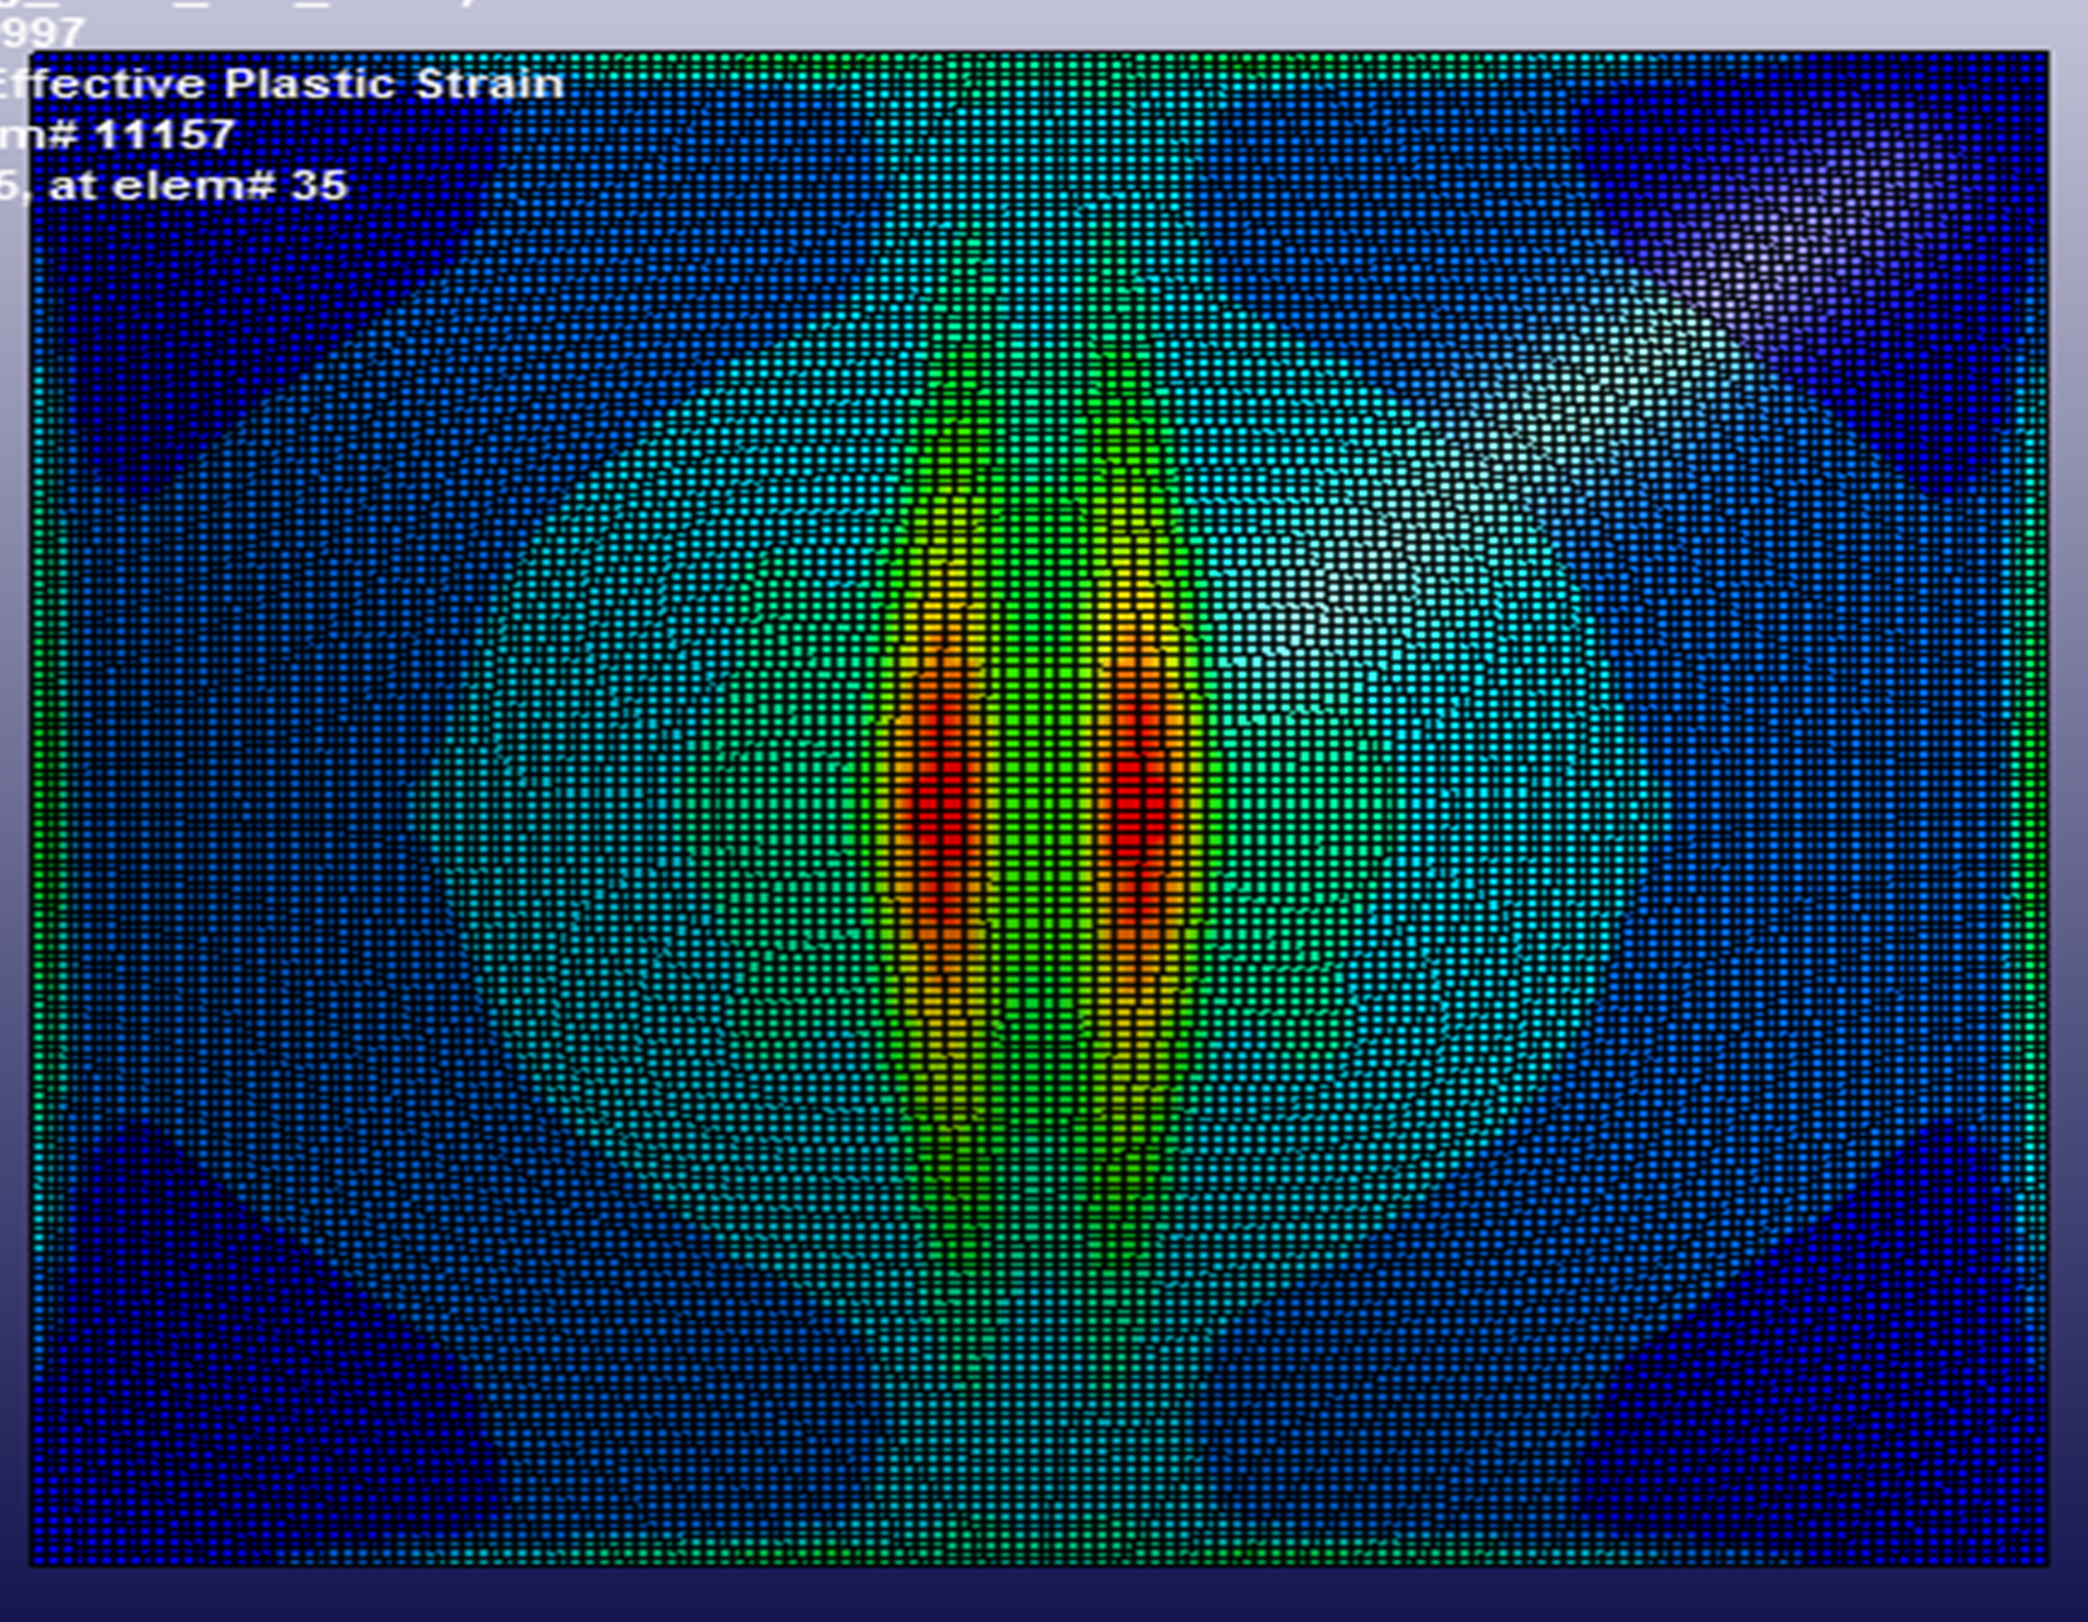
\includegraphics[width=1\linewidth]{DoubleStrainPredict}
	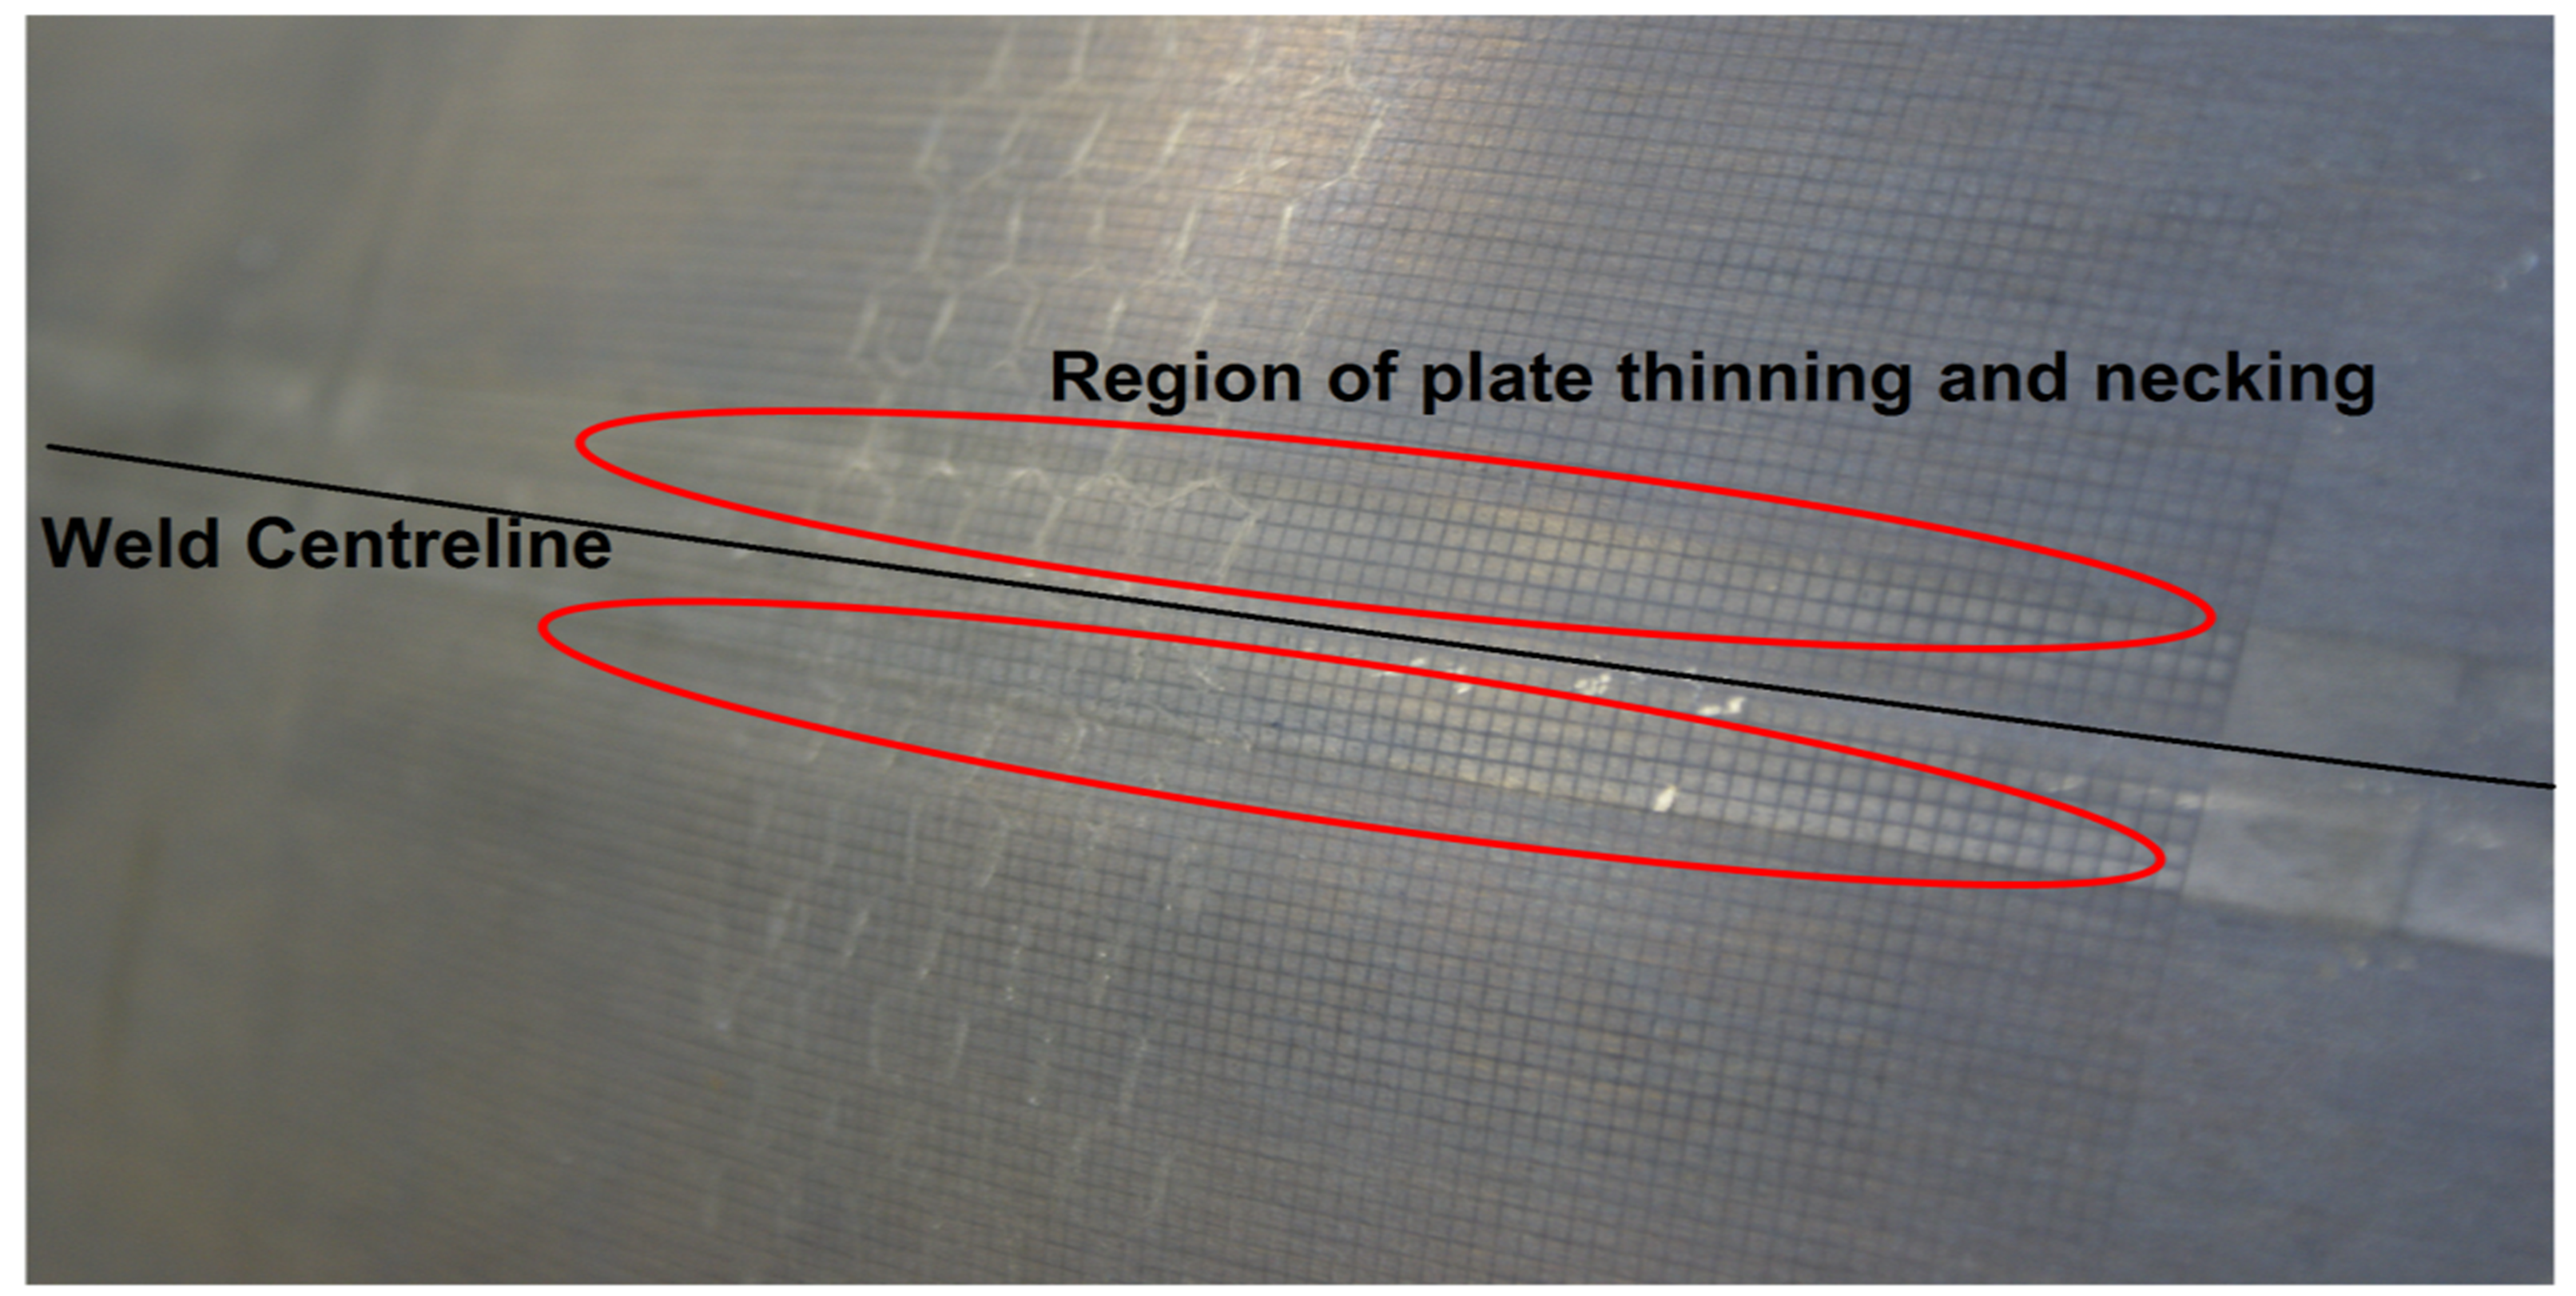
\includegraphics[width=1\linewidth]{DoubleStrainTest}
	\caption[Mesh]{a) Example of the double strain localisation effect predicted under blast loading. b) Observed thinning in welded plates subjected to blast loading which occurs in two locations either side of the weld centreline.}
	\label{fig:BlastStrainReality}
	%TODO Image should say 0.1 microsecong time step NOT 1 microsecond
\end{figure} 
%
%\subsection{Material Property Definition}
%\label{RADMaterialPropertyDefintion}
%Important to have good definition of weld zone properties. This will be addressed specifically in Part II.


% % % % % % % % % % % % % % % % % % % % % % % % % % % % % % % % % % % % % % % % % % % % % % % % % %
% % % % Conclusions
% % % % % % % % % % % % % % % % % % % % % % % % % % % % % % % % % % % % % % % % % % % % % % % % % %
\section{Conclusions}
\label{Conclusion}
In this study, an FE based modelling method, which incorporates element-wise material property variation to detail the strong material property gradients arising from the welding process, was utilised to predict the structural response of FSW 2139-T8 under complex loading configurations, including blast loading. The method requires an understanding of the strengthening mechanism variation in FSW 2139-T8 and is only feasible through automation of the mesh building process. The method utilised removes the need to calibrate models geometry to a particular loading configuration, rather it is calibrated to a normalised weld condition; this removes modelling errors which may arise when extending models to study structural performance under different loading configurations. Moreover, this allows the method to be used to study the effect of welding parameters on structural performance, potentially enabling numerical weld optimisation, which is theoretically applicable to any heat treatable aluminium alloy. The method has been verified experimentally using DIC for FSW 2139-T8 in under uniaxial tension. The method provides good correlation for strain evolution both globally and locally across the weld zone; this represents an improvement over existing techniques reported in the public domain. Furthermore, strong supporting experimental evidence has been generated which indicates that the method provides good qualitative and quantitative correlation with experimental evidence when extended to more complex loading configurations; this represents an improvement on modelling techniques available in the public domain.
%
%\begin{itemize}
%	\item Used FE to predict structural response with variable mat property gradients
%	\item variation in properties linked to strengthening mechanism variation
%	\item understanding mechanism variation has allowed detailed property gradients to be implemented using an automated mesh building process
%	\item We utilise a method whereby you remove calibration wrt loading configuration, rather to a normalised weld condition using Johnson Cook material models. Theoretically you can apply this to any weld.
%	\item the method accurately predicts behaviour in simple loading configurations and has been verified using DIC. In comparision to literature, there is both global and local quantitative correlation of strain evolution (geometrically and spatially)
%	\item method can be extended to complex structures and loading and provides good quantitative correlation with experimental evidence though a more detailed analysis using DIC may provide better data. Improvement from published literature
%	\item method can potentially provide better assessment of failure criterion as removes errors due to modelling itself
%\end{itemize}
%Basically the methodology is sound. Gives good results. Some issues are specifically addressed in Part II and will assumed to be linked to microstructure.

% % % % % % % % % % % % % % % % % % % % % % % % % % % % % % % % % % % % % % % % % % % % % % % % % %
% % % % Acknowledgements
% % % % % % % % % % % % % % % % % % % % % % % % % % % % % % % % % % % % % % % % % % % % % % % % % %
\section*{Acknowledgements}
\label{Acknowledgements}
The authors acknowledge the funding granted from EPSRC via the Advanced Metallic Systems CDT (EP/L016273/1) at the Universities of Manchester and Sheffield and LATEST2 program (EP/G022402/1). Further the authors acknowledge DSTL for their contribution towards development of the FE method; Constellium for the provision and manufacture of materials; and Blastech for technical support during blast testing. Thanks also to David Strong and Bill Storrey for their contribution towards experimental testing; and Samuel Tammas-Williams, Tomas Brownsmith, Faye McCarthy, and Richard Watson for their assistance in producing this paper. Please contact the corresponding author for access to the original data used in this article.

%TODO Research funded by EPSRC and DSTL.... acknowledge for making the article open source as Sam has done. Further thanks go to whoever proof read this piece of shit.

%% The Appendices part is started with the command \appendix;
%% appendix sections are then done as normal sections
%% \appendix

%% \section{}
%% \label{}

%% If you have bibdatabase file and want bibtex to generate the
%% bibitems, please use
%%

% % % % % % % % % % % % % % % % % % % % % % % % % % % % % % % % % % % % % % % % % % % % % % % % % %
% % % % References
% % % % % % % % % % % % % % % % % % % % % % % % % % % % % % % % % % % % % % % % % % % % % % % % % %
\section*{References}
  \bibliographystyle{elsarticle-num} 
  %Referencing system for in the office....
  \bibliography{C:/Users/mbgm6aab/Documents/AdvancedMetallicSystemsCDT/PhD/Papers/library}
 %Referencing system for home....
  %\bibliography{C:/Users/Public/Documents/AdvancedMetallicSystemsCDT/PhD/Papers/library}


%% else use the following coding to input the bibitems directly in the
%% TeX file.

%\begin{thebibliography}{00}

%% \bibitem{label}
%% Text of bibliographic item

%\bibitem{}

%\end{thebibliography}
\end{document}
\endinput
%%
%% End of file `elsarticle-template-num.tex'.
